\documentclass[10pt,aspectratio=43,mathserif,table]{beamer} 
%设置为 Beamer 文档类型,设置字体为 10pt,长宽比为16:9,数学字体为 serif 风格
\batchmode

\usepackage{graphicx}
\usepackage{animate}
\usepackage{tikz}
\usepackage{hyperref}

%导入一些用到的宏包
\usepackage{amsmath,bm,amsfonts,amssymb,enumerate,epsfig,bbm,calc,color,ifthen,capt-of,multimedia,hyperref}
\usepackage{xeCJK} %导入中文包
\setCJKmainfont{SimHei} %字体采用黑体  Microsoft YaHei

\usetheme{Berlin} %主题
\usecolortheme{sustech} %主题颜色

\usepackage[ruled,linesnumbered]{algorithm2e}

\usepackage{fancybox}
\usepackage{xcolor}
\usepackage{times}
\usepackage{listings}

\usepackage{booktabs}
\usepackage{colortbl}

\newcommand{\Console}{Console}
\lstset{ %
	backgroundcolor=\color{white},   % choose the background color
	basicstyle=\footnotesize\rmfamily,     % size of fonts used for the code
	columns=fullflexible,
	breaklines=true,                 % automatic line breaking only at whitespace
	captionpos=b,                    % sets the caption-position to bottom
	tabsize=4,
	commentstyle=\color{mygreen},    % comment style
	escapeinside={\%*}{*)},          % if you want to add LaTeX within your code
	keywordstyle=\color{blue},       % keyword style
	stringstyle=\color{mymauve}\ttfamily,     % string literal style
	numbers=left, 
	%	frame=single,
	rulesepcolor=\color{red!20!green!20!blue!20},
	% identifierstyle=\color{red},
	language=c
}

\setsansfont{Microsoft YaHei}
\setmainfont{Times New Roman}

\definecolor{mygreen}{rgb}{0,0.6,0}
\definecolor{mymauve}{rgb}{0.58,0,0.82}
\definecolor{mygray}{gray}{.9}
\definecolor{mypink}{rgb}{.99,.91,.95}
\definecolor{mycyan}{cmyk}{.3,0,0,0}

%题目,作者,学校,日期
\title{离散数学基础}
\subtitle{\fontsize{9pt}{14pt}\textbf{函数基础知识}}
\author{中山大学MOOC课程组}
\institute{\fontsize{8pt}{14pt}中山大学计算机学院}
\date{\today}

%学校Logo
%\pgfdeclareimage[height=0.5cm]{sustech-logo}{sustech-logo.pdf}
%\logo{\pgfuseimage{sustech-logo}\hspace*{0.3cm}}

\AtBeginSection[]
{
	\begin{frame}<beamer>
	\frametitle{\textbf{目录}}
	\tableofcontents[currentsection]
\end{frame}
}
\beamerdefaultoverlayspecification{<+->}
% -----------------------------------------------------------------------------
\begin{document}
% -----------------------------------------------------------------------------

\frame{\titlepage}

\section[目录]{}   %目录
\begin{frame}{目录}
\tableofcontents
\end{frame}

\section{基础知识回顾}

\subsection{基本概念}

\begin{frame}{函数、像、原像}
	\begin{block}<0->{函数}
		集合A到B的函数$f$,记为$f:A\rightarrow B$,是笛卡尔积集$A\times B$的子集,且满足对任意$a\in A$,都有且只有唯一的$b\in B$使得$<a,b>\in f$。函数通常也称为\textcolor{red}{\textbf{映射}}。
	\end{block}

	\begin{block}<0->{像、原像}
		由于b存在且唯一,因此记$b=f(a)$,称$b$是$a$在函数$f$下的\textcolor{red}{\textbf{像}},$a$是$b$在函数$f$下的\textcolor{red}{\textbf{原像}}。
	\end{block}
\end{frame}

\begin{frame}{域的相关定义}
	\begin{block}{域}
		对于函数$f:A\rightarrow B$,称$A$是$f$的\textcolor{red}{\textbf{定义域}},而$B$称为$f$的\textcolor{red}{\textbf{陪域}}。特别地,$f(A)$称为$f$的\textcolor{red}{\textbf{值域}}。
	\end{block}
	
	\textcolor{mymauve}{对于某个函数$f$来说,它的值域一定为陪域的子集,而且,我们可以得到:一个映射的值域等于陪域,当且仅当映射为\textbf{满射}。}

\end{frame}

\begin{frame}{取整相关定义}
	\begin{block}<0->{天花板(ceiling)}
		\textcolor{red}{\textbf{天花板函数}} $f(x) = \lceil x \rceil$,是大于等于$x$的最小整数。
	\end{block}
	
	\begin{block}<0->{地板(floor)}
		\textcolor{red}{\textbf{地板函数}} $f(x) = \lfloor x \rfloor$,是小于等于$x$的最小整数。
	\end{block}

	\textcolor{mymauve}{天花板和地板的定义域为实数集,而陪域为整数集。}
\end{frame}

\subsection{函数的性质与运算}

\begin{frame}{单函数、满函数、双函数}
	\begin{block}<0->{单函数}
		陪域$B$的每个元素\textcolor{red}{至多}有定义域$A$的一个函数与之对应。单函数有时也称作\textcolor{red}{\textbf{一对一函数}}。
	\end{block}
	
	\begin{block}<0->{满函数}
		陪域$B$的每个元素至少有定义域$A$的一个元素与之对应。满函数有时也称为\textcolor{red}{\textbf{映上函数}}。
	\end{block}
	
	\begin{block}<0->{双函数}
		一个既是单函数又是满函数的函数是双函数,也称为\textcolor{red}{\textbf{一一对应}}。
	\end{block}
\end{frame}

\begin{frame}{特殊约定}
	\begin{itemize}
		\item<0-> 定义域为空的空函数是单函数,如果陪域也为空,那么认为是双函数。
		\item<0-> 对任意集合$A$,$A$上的恒等函数\textbf{id}$_{A}$是双函数。
	\end{itemize}
\end{frame}

\begin{frame}{复合函数、反函数}
	\begin{block}<0->{复合函数}
		函数$f:A\rightarrow B$和$g:B\rightarrow C$的\textcolor{red}{\textbf{复合}},记为$g\circ f$\;(\textcolor{red}{不是$f\circ g$}),定义为:$$\forall x\in A,g\circ f = g(f(x))$$
	\end{block}

	\begin{block}<0->{反函数}
		如果一个函数$f:A\rightarrow B$\textcolor{red}{是双函数},那么它的逆关系$f^{-1}$也是函数,称为$f$的反函数,且对任意$x\in A,y\in B$,$f^{-1}(y)=x$当且仅当$f(x)=y$。
	\end{block}
\end{frame}

\section{习题讲解}

\begin{frame}{判断关系是否可以构成函数}
	下列哪些关系可以构成函数?
	\begin{itemize}
		\item<0-> \{<$x_{1},x_{2}$>|$x_{1},x_{2}\in \mathbf{N},x_{1}+x_{2}\textless 10$\}
		\item<0-> \{<$y_{1},y_{2}$>|$y_{1},y_{2}\in \mathbf{R},y_{2}=y_{1}^{2}$\}
		\item<0-> \{<$y_{1},y_{2}$>|$y_{1},y_{2}\in \mathbf{R},y_{2}^{2}=y_{1}$\}
	\end{itemize}

	\begin{block}<2->{答案}
		不能、能、不能。
	\end{block}

	\begin{block}<3->{解析}
		\textcolor{red}{函数和关系的区别在于他们的对应法则}。在关系$R$的表达式中,如果$<x,y>\in R$,就说$x$对应到$y$,\textcolor{red}{注意这种对应可以是一对一的、多对一的和一对多的}。但函数不允许一对多的对应,因此判别一个关系是否构成函数,就要检查关系中是否存在一对多的情况。
	\end{block}
\end{frame}

\begin{frame}{函数与关系}
	设$f:A\rightarrow B$是函数,且$S$是$B$上的关系,在$A$上定义关系$R$:$$R=\{(x,y)\in A\times A|(f(x),f(y))\in S\}$$
	试证明:
	\begin{itemize}
		\item<0-> 若$S$是自反关系,则$R$也是自反关系。
		\item<0-> 若$S$是对称关系,则$R$也是对称关系。
		\item<0-> 若$S$是传递关系,则$R$也是传递关系。
	\end{itemize}
\end{frame}

\begin{frame}{函数与关系}
	设$f:A\rightarrow B$是函数,且$S$是$B$上的关系,在$A$上定义关系$R$:$$R=\{(x,y)\in A\times A|(f(x),f(y))\in S\}$$
	
	\begin{block}<1->{自反关系}
		假定$S$是自反的,则对任意$x\in A$,有$<f(x),f(x)>\in S$,从而根据$R$的定义,有$<x,x>\in R$,从而$R$也是自反的。
	\end{block}
	
	\begin{block}<2->{对称关系}
		假定$S$是对称的,则对任意$x,y\in A$,有$<f(x),f(y)>\in S$,由于$S$是对称的,那么$<f(y),f(x)>\in S$,从而根据$R$的定义有$<y,x>\in R$,即$R$也是对称的。
	\end{block}
	
\end{frame}

\begin{frame}{函数与关系}
	设$f:A\rightarrow B$是函数,且$S$是$B$上的关系,在$A$上定义关系$R$:$$R=\{(x,y)\in A\times A|(f(x),f(y))\in S\}$$
	
	\begin{block}{传递关系}
		假定$S$是传递的,则对任意$x,y,z\in A$,若$<x,y>\in R$且$<y,z>\in R$,即$<f(x),f(y)>\in S$且$<f(y),f(z)>\in S$。由于$S$是传递的,因此也有$<f(x),f(z)>\in S$,从而根据$R$的定义,有$<x,z>\in R$,这就表明$R$是传递的。
	\end{block}
	
\end{frame}

\begin{frame}{双射函数的构建}
	对下面给定的集合$A$和$B$,构造从$A$到$B$的双射函数。
	\begin{itemize}
		\item<0-> $A = \mathbf{N},B=\{x|x=2^{y}\wedge y\in \mathbf{N}\}$
		\item<0-> $A=[\frac{\pi}{2},\frac{3\pi}{2}],B=[-1,1]$,都是实数区间
	\end{itemize}

	\begin{block}<2->{答案(不唯一,合理即可)}
		\begin{itemize}
			\item $f:A\rightarrow B,f(x)=2^{x}$
			\item $f:A\rightarrow B,f(x)=sinx$
		\end{itemize}
		
	\end{block}
\end{frame}

\begin{frame}{双射函数的构建技巧分析}
	\begin{columns}[T] % align columns
		\begin{column}<0->{.65\textwidth}
			给定集合$A,B$,如何构造从$A$到$B$的双射?一般可采用如下技巧:
			\begin{itemize}
				\item<2-> 若$A$,$B$都是有穷集合,则可用列元素的方法表示$A$,$B$,然后顺序将$A$中的元素与$B$中的元素建立对应。
				\item<3-> 若$A$,$B$都是实数区间,可以采用直线方程作为从$A$到$B$的双射函数。例如$A=[1,2],B=[2,3]$都是实数区间,先将$A,B$分别标记在直角坐标系的$x,y$轴上,过(1,2)和(2,3)两点的直线方程将$A$中的每个数映射到$B$上,因此该直线方程所代表的一次函数就是从$A$到$B$的双射函数,为$f(x)=x+1$。\textcolor{red}{但对半开半闭区间需注意开端点与开端点对应,闭端点与闭端点对应}。
			\end{itemize}
		\end{column}
		\begin{column}<3->{.40\textwidth}
			\begin{figure}
				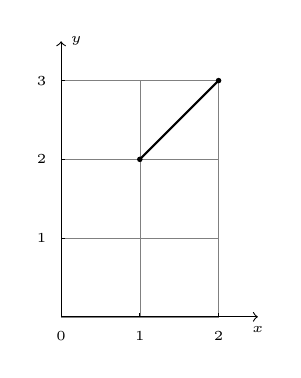
\begin{tikzpicture}
					\draw[step=1,help lines] ( 0,0 ) grid (2, 3);
					\draw[->](0,0)--(2.5,0)node[left,below,font=\tiny]{$x$};
					\draw[->](0,0)--(0,3.5)node[right,font=\tiny]{$y$};
					\foreach \x in {0,1,2}{\draw(\x,0)--(\x,0.05)node[below,outer sep=2pt,font=\tiny]at(\x,0){\x};}
					\foreach \y in {1,2,3}{\draw(0,\y)--(0.05,\y)node[left,outer sep=2pt,font=\tiny]at(0,\y){\y};}
					\draw[color=black, thick,smooth,domain=1:2]plot(\x,\x+1);
					\fill (1,2) circle (1pt);
					\fill (2,3) circle (1pt);
				\end{tikzpicture}
			\end{figure}
		\end{column}
	\end{columns}
\end{frame}

\begin{frame}{双射函数的构建技巧分析}
	\begin{itemize}
		\item<1-> 若$A$是一个无穷集合,而$B$是自然数集$\mathbf{N}$。为构造从$A$到$B$的双射,只需将$A$中的元素排成一个有序序列,且指定这个序列的初始元素,这就叫把$A$"良序化"。例如$A$良序化后为$\{x_{0}.x_{1},x_{2}\cdots\}$,那么令$f:A\rightarrow B,f(x_{i})=i,i=0,1,2,\cdots$,$f$就是从$A$到$B$的双射。
	\end{itemize}
\end{frame}

\begin{frame}{函数性质}
	设$f:A\rightarrow B$和$g:B\rightarrow C$是函数,证明:
	\begin{itemize}
		\item<1-> 如果$g\circ f$是单函数,则$f$是单函数,但$g$不一定是单函数。
		\item<1-> 如果$g\circ f$是满函数,则$g$是满函数,但$f$不一定是满函数。
		\item<1-> 如果$g\circ f$是双函数,则$f$是单函数,且$g$是满函数。
	\end{itemize}
\end{frame}

\begin{frame}{函数性质}
	证明:
	\begin{itemize}
		\item<1-> 设$g\circ f$是单函数,对任意$x_{1},x_{2}\in A$,若$f(x_{1})=f(x_{2})$,则有$g(f(x_{1}))=g(f(x_{2}))$。而由$g\circ f$是单函数可得,$x_{1}=x_{2}$,这就证明了$f$是单函数。
		\item<2-> 设$g\circ f$是满函数,对任意$c\in C$,由于$g\circ f$是满函数,因此一定存在$a\in A$,使得$g\circ f(a)=c$,从而$c$在$g$下有原像$f(a)$,因此$g$为满函数。
		\item<3-> 对于"不一定"的证明,我们通常采用举反例的方法。设$A=\{1,2\},B=\{a,b,c\},C=\{0,1\}$,$f$定义为$f(1)=a,f(2)=b$,$g$定义为$g(a)=g(b)=0,g(c)=1$,即可举出以上两问的反例。
		\item<4-> 由前两问可立即得出第三问的结论。
	\end{itemize}
\end{frame}

\section{总结}

\begin{frame}{总结}
	\begin{itemize}
		\item<1-> 函数的定义
		\begin{itemize}
			\item<1-> 像、原像
			\item<1-> 定义域、陪域、值域
		\end{itemize}
		\item <1-> 函数的性质和运算
		\begin{itemize}
			\item<1-> 单函数、满函数、双函数
			\item<1-> 复合函数、反函数
		\end{itemize}
	\end{itemize}
\end{frame}

\begin{frame}{Thank you}
\begin{center}
\begin{minipage}{1\textwidth}
	\setbeamercolor{mybox}{fg=white, bg=black!50!blue}
 \begin{beamercolorbox}[wd=0.70\textwidth, rounded=true, shadow=true]{mybox}
\LARGE \centering Thank you for listening!  %结束语
\end{beamercolorbox}
 \end{minipage}
\end{center}
\end{frame}


% -----------------------------------------------------------------------------
\end{document}
%文档结束